% Section content template for individual Educative lessons
% This file contains the actual content for a specific section
% Generated from Educative API section content

% Section: Design of a Monitoring System
% Section ID: 5485445638520832
% Section Slug: design-of-a-monitoring-system
% Generated: 2025-12-07T18:38:06.274999

\subsection{Requirements}\label{vC-7faWFJGSRNhYEgDjD-}
\\
Let's sum up what we want our monitoring system to do for us:

\begin{itemize}
\item
\protect\phantomsection\label{0X6V1zVvkLr4SCAQrPxzI}
Monitor critical local processes on a server for crashes.
\item
\protect\phantomsection\label{ljpgdGrb1wVBI9uJwV_vi}
Monitor any anomalies in the use of CPU/memory/disk/network bandwidth by a process on a server.
\item
\protect\phantomsection\label{pzw8jucHMi1wggN8iCa7z}
Monitor overall server health, such as CPU, memory, disk, network bandwidth, average load, and so on.
\item
\protect\phantomsection\label{It9VTSiUON_sIcEUPvg3z}
Monitor hardware component faults on a server, such as memory failures, failing or slowing disk, and so on.
\item
\protect\phantomsection\label{Qcqazy6i_oCZeu_kP0ciQ}
Monitor the server's ability to reach out-of-server critical services, such as network file systems and so on.
\item
\protect\phantomsection\label{tBulU0MPHkfCCc06nqGCU}
Monitor all network switches, load balancers, and any other specialized hardware inside a data center.
\item
\protect\phantomsection\label{JxWPI8XeDHpmXm__Wpqd8}
Monitor power consumption at the server, rack, and data center levels.
\item
\protect\phantomsection\label{nGC5GTMWbCtxInor3-47D}
Monitor any power events on the servers, racks, and data center.
\item
\protect\phantomsection\label{gd5-ln66drN6b28nFF1SQ}
Monitor routing information and DNS for external clients.
\item
\protect\phantomsection\label{ihTkXGEXaNLglrhnUFT4K}
Monitor network links and paths' latency inside and across the data centers.
\item
\protect\phantomsection\label{mVVJHNL62n6bf5c-p09Av}
Monitor network status at the peering points.
\item
\protect\phantomsection\label{Xha4fi34bnm6ILtOfKi4h}
Monitor overall service health that might span multiple data centers---for example, a CDN and its performance.
\end{itemize}
\\
We want automated monitoring that identifies an anomaly in the system and informs the alert manager or shows the progress on a dashboard. Cloud service providers provide a health status of their services:

\begin{itemize}
\item
\protect\phantomsection\label{dW09Ocnbh7Bxk-Qk6KAOR}
AWS: \url{https://health.aws.amazon.com/health/status}
\item
\protect\phantomsection\label{wSh-rTbB1RInqUBbAM4Hv}
Azure: \url{https://status.azure.com/en-us/status}
\item
\protect\phantomsection\label{s0nZUO7EheyJzIkENvy3j}
Google: \url{https://status.cloud.google.com/}
\end{itemize}
\\
You can view the AWS service health dashboard {[} here{]}(https://status.aws.amazon.com/). -\/-\textgreater{}
\\
In a distributed system, why is a dedicated monitoring solution necessary instead of simply relying on individual server logs?
\\
State your reasoning in the widget below.

\textbf{Question:}

Why do you need a dedicated monitoring service?

\textbf{Reference Answer:}

Reason 1. Centralized visibility across the entire system. Reason 2. Detecting correlations and patterns that individual logs would miss. Reason 3. Proactive alerts and faster troubleshooting.

% \vspace{-1.0\baselineskip}
\noindent
\begin{minipage}[t]{0.48\textwidth}\vspace{0pt}

\end{minipage}
\hfill
\begin{minipage}[t]{0.48\textwidth}\vspace{0pt}

\end{minipage}

\subsection{Building blocks we will use}\label{2e1DKxIbbJbm2eEchX2Cr}
\\
The design of distributed monitoring will consist of the following building block:

\begin{figure}[htbp]
 \centering
 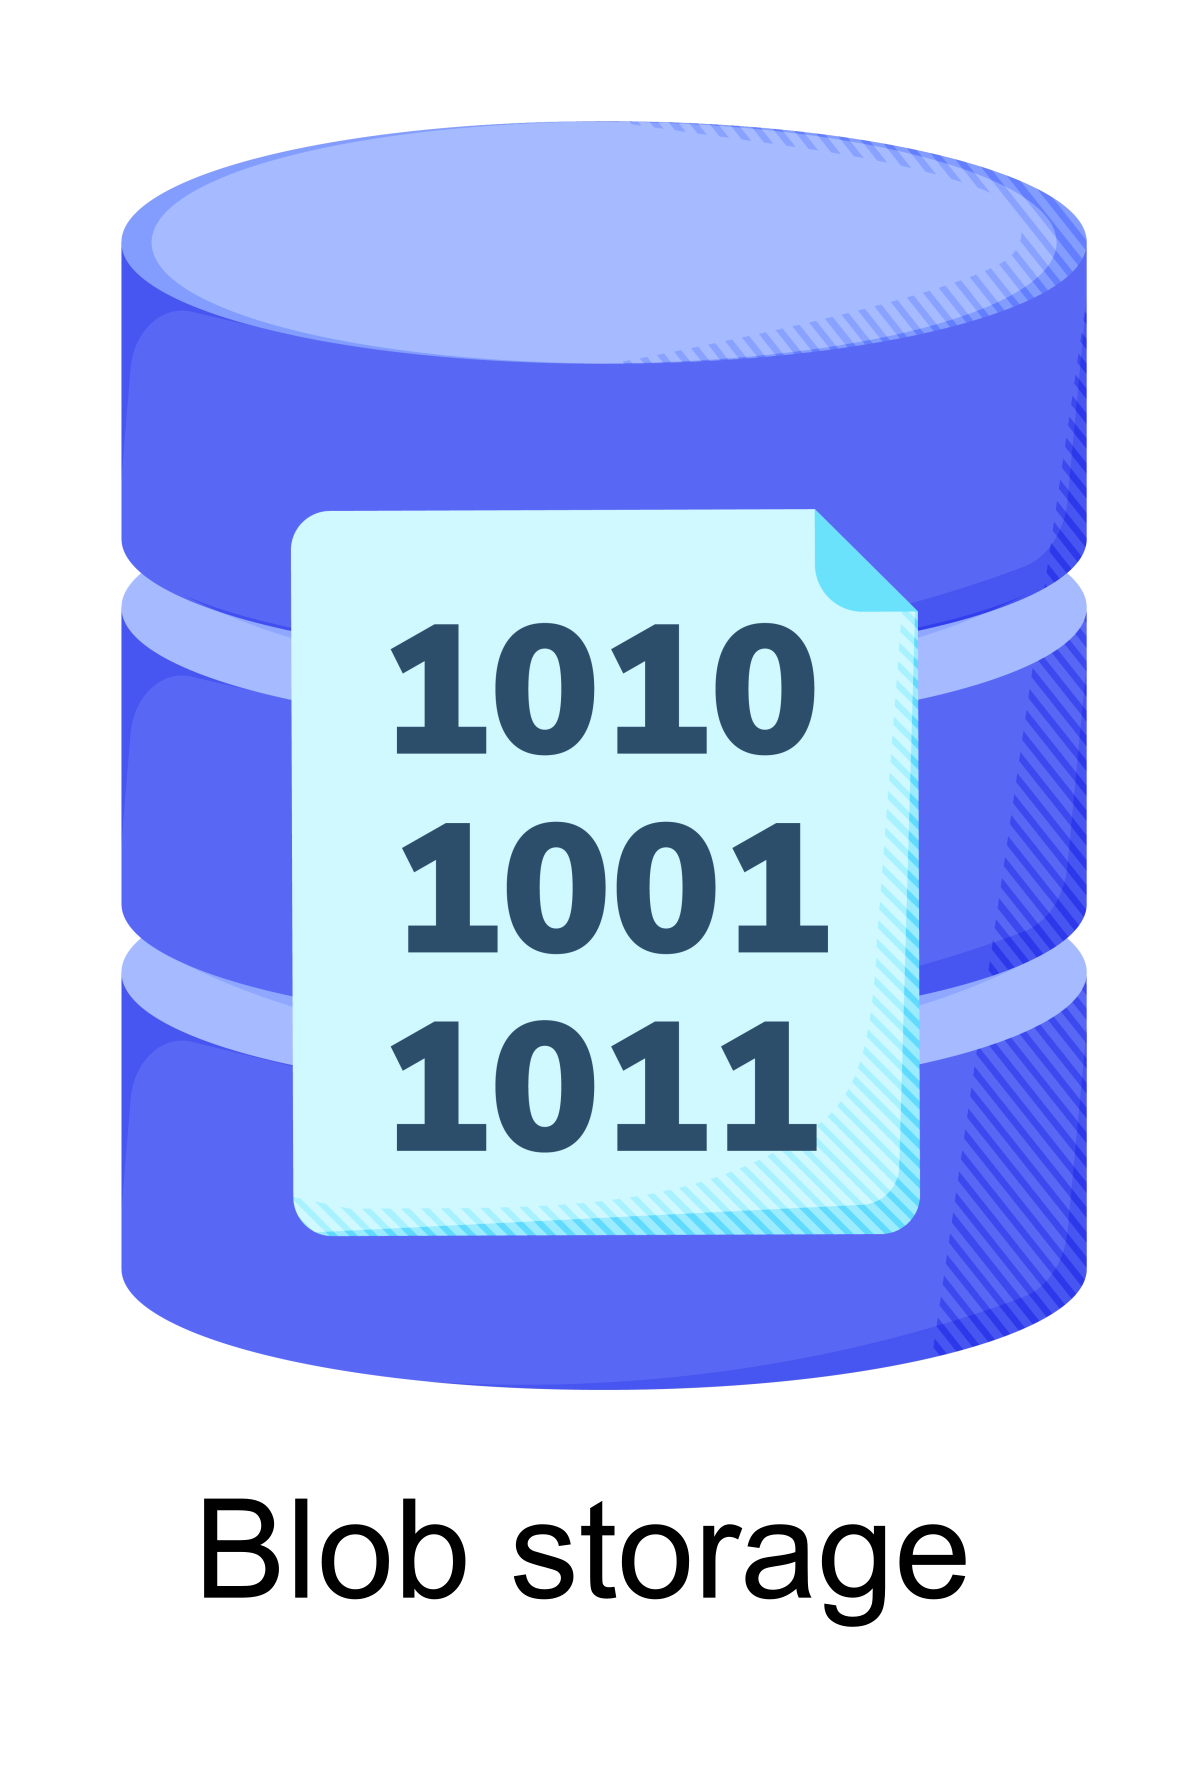
\includegraphics[width=0.2\textwidth]{Images/chapter_14/section_5485445638520832/5369882319126528.png}
 
\end{figure}

\href{https://www.educative.io/courses/grokking-the-system-design-interview/system-design-a-blob-store}{\textbf{Blob storage}}: We'll use blob storage to store our information about metrics.

\subsection{High-level design}\label{E9IGygi62J-_Os4CtbS9S}
\\
The high-level components of our monitoring service are the following:

\begin{itemize}
\item
\protect\phantomsection\label{G2LEVl2UbN8M6TucRhYaL}
\textbf{Storage}: A time-series database stores metrics data, such as the current CPU use or the number of exceptions in an application.
\item
\protect\phantomsection\label{6-xOxQIp5Tlmigt3EJXVy}
\textbf{Data collector service}: This fetches the relevant data from each service and saves it in the storage.
\item
\protect\phantomsection\label{FxgGHmqVoMkUVoUpau3hQ}
\textbf{Querying service}: This is an API that can query on the time-series database and return the relevant information.
\end{itemize}

\begin{figure}[htbp]
 \centering
 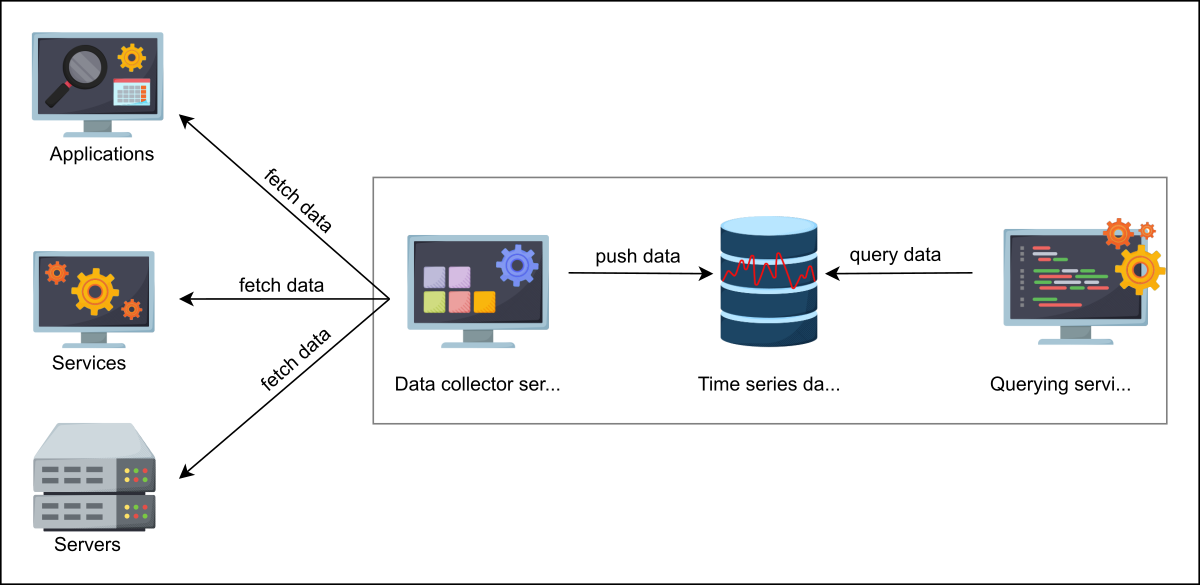
\includegraphics[width=0.5\textwidth]{Images/chapter_14/section_5485445638520832/4549247968346112.png}
 \caption{High-level design of a monitoring system}
\end{figure}

Let's dive deep into the components mentioned above in the next lesson.

% End of section content